\documentclass{article}
\usepackage[utf8]{inputenc}
\usepackage{fullpage}
\usepackage{amsthm,amsmath,amssymb}
\usepackage{tikz}
\usepackage[hidelinks,draft=false,colorlinks=true]{hyperref}
\usepackage[capitalize]{cleveref} % after hyperref!

%%%%%%%%%%%%%%%%%%%%%%%%%%%%%%%%%%%%%%%%%%%%%%%%%%%%%%%%%%%%
%%%% For bibliography
\usepackage[sorting=none, backend=biber, url=false, isbn=false, hyperref=true, eprint=true, maxbibnames=6]{biblatex}
\addbibresource{/home/molnar/Dropbox/ZoteroLibrary.bib}
\AtEveryBibitem{%
	\clearfield{eprintclass}%
}

% Setting title to point to doi link
\ExecuteBibliographyOptions{doi=false}
\newbibmacro{string+doi}[1]{%
	\iffieldundef{doi}{#1}{\href{http://dx.doi.org/\thefield{doi}}{#1}}}
\DeclareFieldFormat{title}{\usebibmacro{string+doi}{\mkbibemph{#1}}}
\DeclareFieldFormat[article]{title}{\usebibmacro{string+doi}{\mkbibquote{#1}}}

%%%%%%%%%%%%%%%%%%%%%%%%%%%%%%%%%%%%%%%%%%%%%%%%%%%%%%%%%%%%
%%% hyperref setup
\hypersetup{
	pdftitle={Tensor Networks},
	pdfauthor={Andras Molnar},
	bookmarks=true,
	bookmarksnumbered=true,
	bookmarksopen=true,
	bookmarksopenlevel=1,
	colorlinks,
	%linkcolor=blue!50!black,
	%urlcolor=cyan!50!black!90,
	pdfstartview=Fit,
	pdfpagemode=UseOutlines,    
	pdfpagelayout=TwoPageRight
}

\newtheorem{lemma}{Lemma}
\newtheorem{fact}{Fact}
\newtheorem{proposition}{Proposition}
\newtheorem{theorem}{Theorem}
\newtheorem{corollary}{Corollary}
\newtheorem{remark}{Remark}
\newtheorem{definition}{Definition}
\newtheorem{exercise}{Exercise}


\newcommand{\tr}{\operatorname{Tr}}
\newcommand{\id}{\mathrm{Id}}
\newcommand{\todo}[1]{{\color{red} #1}}
\newcommand{\myfcn}{nice }
\newcommand{\myfcntwo}{admissible }
\newcommand{\End}{\mathrm{End}}
\newcommand{\ket}[1]{\vert #1 \rangle}
\newcommand{\bra}[1]{\langle #1 \vert}
\newcommand{\scalprod}[2]{\langle #1 \vert #2 \rangle}
\newcommand{\Span}{\mathrm{Span}}


\tikzset{
	tensor/.style={
		inner sep = 0.055cm,
		shape = circle,
		draw,
		fill
	},
	t/.style={
		inner sep = 0.03cm,
		shape = circle,
		draw,
		fill
	},
}

\tikzset{>=stealth}


\title{Tensor Networks}
\author{Andras Molnar}

\begin{document}

\maketitle

\begin{remark}
	In these notes all vector spaces are complex and finite dimensional unless otherwise stated.
\end{remark}


\section{Introduction}

Tensor Networks provide good description for ground states of many-body Hamiltonians that appear in physics. These Hamiltonians are usually defined on a large number of particles (of the order $10^{23}$). To consider such systems one either works directly with an infinite number of particles (thermodynamic (TD) limit), or one considers a series of finite systems that ``approximate the TD limit'' as the size of the system grows. Either way, Hamiltonians that appear are usually local and gapped. In these notes we consider only systems composed of a fixed number of particles that are distinguishable and finite dimensional (``spins''): that is, one particle is described on a finite dimensional Hilbert space $\mathcal{H}$, and $N$ particles are described on the Hilbert space $\mathcal{H}^{\otimes N}$. 

Here locality means the following: particles are arranged in a 1,2 or 3 dimensional space and only particles that are ``close'' to each other interact. That is, the Hamiltonian is a sum of terms $H = \sum_i h_i$, and each term in the sum has the structure $h_i = \id_{\Lambda\backslash S_i} \otimes h_{S_i}$, where $\Lambda$ is the set of all particles (for a given system size), $S_i$ are subsets of particles that are close to each other, $\id_{\Lambda\backslash S_i}$ is the identity in $\bigotimes_{j \in \Lambda\backslash S_i}\mathcal{B}(\mathcal{H}_j)$ and $h_{S_i}\in\bigotimes_{j\in S_i} \mathcal{B}(\mathcal{H}_j)$. As the system size $|\Lambda| = N$ grows, $|S_i|$ stays bounded, but the number of terms in the Hamiltonian grow linearly with $N$.

We call a Hamiltonian gapped if the difference between the lowest and second lowest eigenvalue stays above a constant as the system size $N$ tends to infinity. Given a path of gapped Hamiltonians, one can show that expectation values of local observables change continuously, i.e., gap provides stability against perturbations. 


Given a many-body Hamiltonian, a general goal is to understand its ground state. While the ground state is just simply the lowest energy eigenvector of the Hamiltonian, finding it is difficult for large system sizes. In fact, for $N$ large enough, one cannot store the full matrix of the Hamiltonian on the computer, and neither can one store the description of the state expanded in the computational basis. 

Tensor networks provide a way to approximate ground states of gapped local Hamiltonians and to calculate expectation values and correlations of local observables. 
 
\section{Matrix Product States (MPS)}

\begin{definition}[MPS]
  Let $V$ be a vector space and $\mathcal{H}$ be a Hilbert space with basis $\mathcal{B} = \{\ket{0},\ket{1},\dots \ket{d-1}\}$. A tensor $A\in \End(V)\otimes \mathcal{H}$, $A = \sum_{i\in \mathcal{B}} A_i \otimes \ket{i}$ is called an MPS tensor. The translation invariant (TI) MPS on $n$ sites is a state $\mathfrak{M}_n(A)\in \mathcal{H}^{\otimes n}$ defined by
  \begin{equation*}
  	\mathfrak{M}_n(A) = \sum_{i\in \mathcal{B}^n} \tr\left\{A_{i_1} A_{i_2} \dots A_{i_n}\right\} \ket{i_1 i_2 \dots i_n}.
  \end{equation*}
  We call $V$ the bond space and $\dim(V)$ the bond dimension of the MPS.
\end{definition}

A class of MPS, called injective MPS, is going to play a crucial role in the theory of MPS. We will prove that any TI MPS -- after blocking -- decomposes into a sum of injective MPS. The parent Hamiltonian of an injective MPS is gapped and the MPS is its unique ground state. Two injective MPS are either orthogonal in the thermodynamic limit or are generating the same state for all system sizes. If they generate the same state for a large enough system size, then the two MPS tensors are related to each other by a gauge transformation. 

We will use all these statements to understand the classification of phases in 1D spin systems, with and without symmetries. 

To define injective MPS, we introduce MPS with arbitrary boundary condition:
\begin{definition}[MPS with boundary]
  Let $V$ be a vector space and $\mathcal{H}$ be a Hilbert space with basis $\mathcal{B} = \{\ket{0},\ket{1},\dots \ket{d-1}\}$. A tensor $A\in \End(V)\otimes \mathcal{H}$, $A = \sum_{i\in \mathcal{B}} A_i \otimes \ket{i}$ is called an MPS tensor. The MPS on $n$ sites with a given boundary condition $X$ is a state $\mathfrak{M}_n(A,X)\in \mathcal{H}^{\otimes n}$ defined by
  \begin{equation*}
    \mathfrak{M}_n(A,X) = \sum_{i\in \mathcal{B}^n} \tr\left\{XA_{i_1} A_{i_2} \dots A_{i_n}\right\} \ket{i_1 i_2 \dots i_n}.
  \end{equation*}
\end{definition}

Notice that the periodic boundary condition MPS $\mathfrak{M}_n(A)$ can also be written as $\mathfrak{M}_n(A) = \mathfrak{M}_n(A,\id)$.

\begin{definition}[Injective MPS]
  Let $V$ be a vector space and $\mathcal{H}$ be a Hilbert space. An MPS tensor $A\in \End(V)\otimes \mathcal{H}$ is called \emph{injective} if $\exists n\in\mathbb{N}$ s.t the map $X\mapsto \mathfrak{M}_n(A,X)$ is injective.
\end{definition}

\begin{theorem}\label{thm:injectivity_equivalent}
  Let $V$ be a vector space and $\mathcal{H}$ be a Hilbert space with basis $\mathcal{B} = \{\ket{0},\ket{1},\dots \ket{d-1}\}$. The MPS tensor $A\in \End(V)\otimes \mathcal{H}$, $A = \sum_{i\in \mathcal{B}} A_i \otimes \ket{i}$, is injective if and only if $\exists n\in \mathbb{N}$ s.t.
  \begin{equation*}
  	\Span\left\{A_{i_1} A_{i_2} \dots A_{i_n} \middle| i\in \mathcal{B}^n \right\} = \End(V).
  \end{equation*}
\end{theorem}

\begin{proof}
	Let $S_n = \Span\left\{A_{i_1} A_{i_2} \dots A_{i_n} \middle| i\in \mathcal{B}^n \right\}$. Notice that $\mathfrak{M}_n(A,X)=0$ is equivalent to $\tr\{XY\} = 0$ $\forall Y\in S_n$.
  
  Assume now that $S_n = \End(V)$. Then $\mathfrak{M}_n(A,X) = 0$ is equivalent to $\tr \{XY\} = 0 $ $\forall Y\in \End(V)$. As the bilinear functional $(X,Y)\mapsto \tr (XY)$ is non-degenerate, this implies $X=0$, i.e.\ the MPS is injective.
  
  For the other direction, we need to show that $S_n\subsetneq \End(V)$ implies that $A$ is not injective. As the bilinear functional $(X,Y)\mapsto \tr (XY)$ is non-degenerate, $\exists X\neq 0$ such that $\tr (XY) = 0 \ \forall Y\in S_n$, and thus $\mathfrak{M}_n(A,X) = 0$, i.e.\ the MPS is not injective.
\end{proof}


\begin{theorem}
  Let $V$ be a vector space and $\mathcal{H}$ be a Hilbert space, and let $A\in \End(V)\otimes \mathcal{H}$ be an MPS tensor. Then, if $X\mapsto\mathfrak{M}_n(A,X)$ is injective for some $n\in\mathbb{N}$, then $X \mapsto \mathfrak{M}_k(A,X)$ is injective as well for any $k\geq n$.
\end{theorem}

\begin{proof}
  Let $S_n = \Span\left\{A_{i_1} A_{i_2} \dots A_{i_n} \middle| i\in \mathcal{B}^n \right\}$. Using \cref{thm:injectivity_equivalent}, $\psi_n$ is injective if and only if $S_n = \End(V)$. It is enough to show thus that if $S_n = \End(V)$, then $S_{n+1} = \End(V)$ as well. Notice that $S_{n+1} = \Span\{S_1 S_n\} = \Span\{ S_1 \End(V)\}$, and that $S_{n} = \Span\{S_1 S_{n-1}\} \subseteq \Span\{S_1 \End(V)\}$. Therefore $S_{n+1} \supseteq S_n = \End(V)$, i.e.\ $S_{n+1} = \End(V)$. 
\end{proof}

\begin{definition}[Injectivity length]
    Let $V$ be a vector space and $\mathcal{H}$ be a Hilbert space. Let $A\in \End(V)\otimes \mathcal{H}$ be an \emph{injective} MPS tensor. The minimal $n$ for which the map $X\mapsto \mathfrak{M}_n(A,X)$ is injective is called the \emph{injectivity length} of $A$.
\end{definition}

\begin{lemma}\label{lem:injective_l_r_inverse}
  Let $V$ be a vector space and $\mathcal{H}$ be a Hilbert space with basis $\mathcal{B} = \{\ket{0},\ket{1},\dots \ket{d-1}\}$. Let $A\in \End(V)\otimes \mathcal{H}$, $A = \sum_{i\in \mathcal{B}} A_i \otimes \ket{i}$, be an injective tensor. Then there are $l_j\in \End(V)$ and $r_j \in \End(V)$ ($j\in\mathcal{B}$) such that
  \begin{equation*}
    \sum_j A_j r_j = \sum_j l_j A_j = \id.
  \end{equation*} 
\end{lemma}
\begin{proof}
  Injectivity of $A$ implies that there is $n\in\mathbb{N}$ such that $\id\in\End(V) = \Span\left\{A_{i_1} A_{i_2} \dots A_{i_n} \middle| i\in \mathcal{B}^n \right\}$, that is, there is  $c_{i_1\dots i_n}$ such that $\sum_i c_{i_1 \dots i_n} A_{i_1}\dots A_{i_n} = \id$. We can thus set $r_j = \sum_{i_2 \dots i_n} c_{ji_2\dots i_n} A_{i_2}\dots A_{i_n}$ and $l_j = \sum_{i_1 \dots i_{n-1}} c_{i_1\dots i_{n-1}j} A_{i_1}\dots A_{i_{n-1}}$. 
\end{proof}



\begin{remark}
  Let $V_A, V_B$ be two vector spaces and $\mathcal{H}$ be a Hilbert space with basis $\mathcal{B} = \{\ket{0},\ket{1},\dots \ket{d-1}\}$. Let $A\in \End(V_A)\otimes \mathcal{H}$, $A = \sum_{i\in \mathcal{B}} A_i \otimes \ket{i}$, and $B\in \End(V_B)\otimes \mathcal{H}$, $B = \sum_{i\in \mathcal{B}} B_i \otimes \ket{i}$, be two MPS tensors, such that 
  \begin{equation}\label{eq:gauge_1}
    B_i = X A_i X^{-1} \quad \forall i = \{0,1,\dots d-1\}.
  \end{equation}
  Then for all $n\in\mathbb{N}$, $\mathfrak{M}_n(A) = \mathfrak{M}_n(B)$.
\end{remark}

\begin{proof}
  \begin{equation*}
    \mathfrak{M}_n(B) = \sum_{i\in \mathcal{B}^n} \tr\left\{B_{i_1} B_{i_2} \dots B_{i_n}\right\} \ket{i_1 i_2 \dots i_n}.
  \end{equation*}
  Using now \cref{eq:gauge_1}, we obtain   
  \begin{equation*}
    \mathfrak{M}_n(B) = \sum_{i\in \mathcal{B}^n} \tr\left\{XA_{i_1}X^{-1} XA_{i_2}X^{-1} \dots XA_{i_n}X^{-1}\right\} \ket{i_1 i_2 \dots i_n}.
  \end{equation*}
  Noticing that between two MPS tensors $X^{-1}X=\id$ (and using cyclicity of the trace), we directly obtain  that $\mathfrak{M}_n(B) = \mathfrak{M}_n(A)$.
\end{proof}

Under certain conditions the statement can be reversed: if two MPS tensors $A$ and $B$ generate the same state, then they are related to each other via \cref{eq:gauge_1}. 


\begin{theorem}[Fundamental theorem of injective MPS]\label{thm:fundamental}
    Let $V_A, V_B$ be two vector spaces and $\mathcal{H}$ be a Hilbert space with basis $\mathcal{B} = \{\ket{0},\ket{1},\dots \ket{d-1}\}$. Let $A\in \End(V_A)\otimes \mathcal{H}$, $A = \sum_{i\in \mathcal{B}} A_i \otimes \ket{i}$, and $B\in \End(V_B)\otimes \mathcal{H}$, $B = \sum_{i\in \mathcal{B}} B_i \otimes \ket{i}$, be two injective MPS tensors such that both of their injectivity length is at most $n$. If $\mathfrak{M}_k(A) = \mathfrak{M}_k(B)$ for some $k\geq 2n+1$,  then $\exists X: V_B \leftarrow V_A$ invertible, unique up to a multiplicative constant, such that 
    \begin{equation*}
       B_i = X A_i X^{-1}, \quad \forall i = \{0,1,\dots d-1\}.
    \end{equation*}
\end{theorem}

\begin{proof}
  Let us write $\mathfrak{M}_k(A) = \mathfrak{M}_k(B)$ explicitly:
  \begin{equation*}
    \sum_{i\in \mathcal{B}^k} \tr\left\{A_{i_1} A_{i_2} \dots A_{i_k}\right\} \ket{i_1 i_2 \dots i_k} = 
    \sum_{i\in \mathcal{B}^k} \tr\left\{B_{i_1} B_{i_2} \dots B_{i_k}\right\} \ket{i_1 i_2 \dots i_k}
  \end{equation*}
  Let us write $k = n+l$ with $l\geq n+1$ and bipartition the indices in this equation accordingly:
  \begin{equation}\label{eq:ft_thm_1}
    \sum_{\substack{i\in \mathcal{B}^n\\j\in\mathcal{B}^l}} \tr\left\{A_{i_1} \dots A_{i_n} A_{j_1} \dots A_{j_l}\right\} \ket{i_1 \dots i_n} \ket{j_1 \dots j_l}= 
    \sum_{\substack{i\in \mathcal{B}^n\\j\in\mathcal{B}^l}} \tr\left\{B_{i_1} \dots B_{i_n} B_{j_1} \dots B_{j_l}\right\} \ket{i_1 \dots i_n} \ket{j_1 \dots j_l}.
  \end{equation}
  Let $X\in \End(V_A)$ be arbitrary. From the injectivity of the tensor $A$, using \cref{thm:injectivity_equivalent}, we obtain that there is a linear functional $f:\mathcal{H}^{\otimes n}\to \mathbb{C}$ such that 
  \begin{equation*}
    X = \sum_{i\in\mathcal{B}^n} A_{i_1} \dots A_{i_n} \cdot \scalprod{f}{i_1 \dots i_n}.
  \end{equation*}
  Let us fix this $f$ and write 
  \begin{equation*}
    Y = \sum_{i\in\mathcal{B}^n} B_{i_1} \dots B_{i_n} \cdot \scalprod{f}{i_1 \dots i_n}, \quad Y\in\End(V_B).
  \end{equation*}
  Applying the linear map $f\otimes\id: \mathcal{H}^{\otimes n} \otimes \mathcal{H}^{\otimes l} \to \mathcal{H}^{\otimes l}$ on \cref{eq:ft_thm_1} we conclude thus that
  \begin{equation*}
    \sum_{j\in\mathcal{B}^l} \tr\left\{X A_{j_1} \dots A_{j_l}\right\} \ket{j_1 \dots j_l}= 
    \sum_{j\in\mathcal{B}^l} \tr\left\{Y B_{j_1} \dots B_{j_l}\right\} \ket{j_1 \dots j_l}.
  \end{equation*}
  Because of the injectivity of the MPS tensor $B$, $Y$ is uniquely defined. As $X$ was arbitrary, we conclude that for all $X\in \End(V_A)$ there is a unique $Y\in \End(V_B)$ such that this equation holds. Exchanging the role of $A$ and $B$ we obtain that also for all $Y\in \End(V_B)$ exists a unique $X\in \End(V_A)$ such that this equation holds, and thus $X\mapsto Y$ is invertible. Let $f: X\mapsto Y$ be the corresponding map. Notice that $f: \End(V)\to \End(V)$ is linear. As $\End(V)\simeq V\otimes V^*$, we can think of this map as $f\in \End(V)\otimes \End(V^*)$. Let $f = \sum_{i=1}^r L_i \otimes R_i^T$ be the Schimdt decomposition corresponding to this tensor product (in particular, the sets $\{L_i\}_{i=1\dots r}$ and $\{R_i\}_{i=1\dots r}$ are linearly independent). That is, $f$ acts as $Y = \sum_i L_i X R_i$, and thus  
  \begin{equation*}
    \sum_{j\in\mathcal{B}^l} \tr\left\{X A_{j_1} \dots A_{j_l}\right\} \ket{j_1 \dots j_l}= 
    \sum_{j\in\mathcal{B}^l,i} \tr\left\{L_i X R_i B_{j_1} \dots B_{j_l}\right\} \ket{j_1 \dots j_l}, \quad \forall X\in \End(V_A).
  \end{equation*}
  Setting $X=\id$ we observe that $\sum_i L_i R_i\neq 0$. Through non-degeneracy of the trace, we conclude that
  \begin{equation}\label{eq:ft_thm_2}
    \sum_{j\in\mathcal{B}^l}  A_{j_1} \dots A_{j_l} \otimes  \ket{j_1 \dots j_l}= 
    \sum_{j\in\mathcal{B}^l,i}  R_i B_{j_1} \dots B_{j_l}L_i \otimes \ket{j_1 \dots j_l}.
  \end{equation}
  Let us repeat the same argument as above, but decomposing $k$ as $(n+1)+(l-1)$. We obtain that there is $\sum_i \hat R_i \otimes \hat L_i$ such that $\sum_i \hat L_i \hat R_i \neq 0$ and    
  \begin{equation*}
    \sum_{j\in\mathcal{B}^l}  A_{j_1} \dots A_{j_{l-1}} \otimes  \ket{j_1 \dots j_{l-1}}= 
    \sum_{j\in\mathcal{B}^l,i}  \hat R_i B_{j_1} \dots  B_{j_{l-1}} \hat L_i \otimes \ket{j_1 \dots j_{l-1}}.
  \end{equation*}
  Substituting this back in \cref{eq:ft_thm_2}, once for the first $l-1$ spins and once for the last $l-1$ spins, we obtain
  \begin{equation*}
      \sum_{j\in\mathcal{B}^l}  A_{j_1} \hat R_i B_{j_2} \dots B_{j_l} \hat L_i  \otimes  \ket{j_1 \dots j_l}= 
    \sum_{j\in\mathcal{B}^l}  \hat R_i B_{j_1} \dots B_{j_{l-1}} \hat L_i A_{j_l} \otimes  \ket{j_1 \dots j_l}= 
      \sum_{j\in\mathcal{B}^l,i}  R_i B_{j_1} \dots B_{j_l}L_i \otimes \ket{j_1 \dots j_l}.
  \end{equation*}
  Using that $l-1\geq n$ and injectivity of the MPS tensor $B$, we obtain
  \begin{align}
    \sum_i R_i \otimes B_j L_i = \sum_i \hat R_i \otimes \hat L_i A_j \quad \forall j, \label{eq:ft_LR1}\\
    \sum_i R_i B_j \otimes L_i = \sum_i A_j \hat R_i \otimes \hat L_i \quad \forall j \label{eq:ft_LR2}.
  \end{align}
  Let us use \cref{lem:injective_l_r_inverse} for the tensor $B$ together with the first equation:
  \begin{equation*}
     \sum_{i} R_i \otimes L_i =  \sum_{ij} R_i \otimes l_jB_j L_i = \sum_{ij} \hat R_i \otimes l_j\hat L_i A_j.
  \end{equation*}
  Let us argue now that linear independence of $L_i$ implies that $\Span\{R_i\} \subseteq \Span\{\hat R_i\}$: due to the linear independence, we can find linear functionals $\lambda_k: \End(V)\to \mathbb{C}$ such that $\lambda_k(L_i) = \delta_{ik}$. Applying thus $\lambda_k$ on the second component of the tensor product, we obtain that 
  \begin{equation*}
    R_k = \sum_{i} R_i \cdot \lambda_k(L_i) =  \sum_{i} \hat R_i \cdot \lambda_k\left(\sum_j l_j\hat L_i A_j \right) = \sum_{ik} \mu_{ki} \hat R_i,
  \end{equation*}
  for some $\mu_{ki} \in \mathbb{C}$, i.e., $\Span\{R_i\} \subseteq \Span\{\hat R_i\}$. The same way, using \cref{lem:injective_l_r_inverse} for the tensor $A$  leads to the conclusion that $\Span\{R_i\} \supseteq \Span\{\hat R_i\}$, and thus $\Span\{R_i\} = \Span\{\hat R_i\}$. Similarly, from the second equation, we conclude then that $\Span\{L_i\} = \Span\{\hat L_i\}$. Therefore \cref{eq:ft_LR1,eq:ft_LR2} imply that there is an automorphism $L\mapsto \hat{L}$ of $\Span\{L_i\}$ and an automorphism $R\mapsto \hat{R}$ of $\Span\{R_i\}$ such that 
  \begin{align}
    B_jL = \hat{L}A_j \quad \forall j \in \mathcal{B}, \label{eq:ft_main1}\\
    A_jR = \hat R B_j \quad \forall j \in \mathcal{B} \label{eq:ft_main2}
  \end{align}  
  Combining these two equations, we conclude that
  \begin{align*}
    B_j LR = \hat L A_j R = \hat L \hat R B_j \quad \forall j\in\mathcal{B},\\
    A_j RL = \hat R B_j L = \hat R \hat L A_j \quad \forall j\in\mathcal{B}.
  \end{align*}
  Iterating this equation we conclude that for any $L\in\Span\{L_i\}$ and $R\in\Span\{R_i\}$ there is $ \hat{L} \in \Span\{L_i\}$ and  $\hat{R} \in \Span\{R_i\}$ such that 
  \begin{align*}
    B_{j_1} \dots B_{j_n} LR = \hat L \hat R B_{j_1} \dots B_{j_n} \quad \forall j\in\mathcal{B}^n, \\
    A_{j_1} \dots A_{j_n} RL = \hat R \hat L A_{j_1} \dots A_{j_n} \quad \forall j\in\mathcal{B}^n.
  \end{align*}
  Injectivity of the tensors $A$ and $B$ imply then that for all 
  \begin{align*}
    X LR = \hat L \hat R X \quad \forall X\in \End(V_B) \\
    Y RL = \hat R \hat L Y \quad \forall Y\in \End(V_A),
  \end{align*}
  This directly implies that $LR = \hat{L}\hat{R} \propto \id_{V_B}$, and thus $LR\propto \id_{V_B}$ for any $L\in\Span\{L_i\}$ and $R\in \Span\{R_i\}$. Similarly, $RL\propto \id_{V_A}$ for any $L\in\Span\{L_i\}$ and $R\in \Span\{R_i\}$.  As $\sum_i L_i R_i \neq 0$, there is $L\in \Span\{L_i\}$ and $R\in \Span\{R_i\}$ such that $LR\neq 0$. This means that $RL\neq 0$ neither, and thus $L$ is invertible. As $LR \propto \id$ for all $R\in \Span\{R_i\}$, this implies that $R\propto L^{-1}$, and thus $\Span\{R_i\}$ is one dimensional (spanned by $L^{-1}$), so $\Span\{L_i\}$ is also one dimensional, spanned by $L$. Finally \cref{eq:ft_main1} implies that $B_j = LA_j L^{-1}$.
\end{proof}


\paragraph{Examples.} Let us consider some examples where the theorem does NOT apply. We keep the state in the examples simple: we will consider different MPS descriptions of the product state $\ket{0}^{\otimes n}$. These representations will not meet the requirements of \cref{thm:fundamental} as at least one of the MPS tensors is not injective. Consequently, the fundamental theorem does not apply, and in fact, the different MPS tensors are not related to each other by a basis transformation. First, one can consider the ``canonical'' way to represent it as an MPS:
\begin{equation*}
  A_0 = 1, \quad 
  A_1 = 0;
\end{equation*}
again, these matrices are $1\times 1$, the MPS has bond dimension 1. This is an injective MPS description of the state. The same state admits another description that is trivially the same, yet it is non-injective:
\begin{equation*}
  B_0 = \left(\begin{matrix}
    1 & 0 \\ 0 & 0 
  \end{matrix}\right), \quad 
  B_1 = \left(\begin{matrix}
    0 & 0 \\ 0 & 0 
  \end{matrix}\right).
\end{equation*}
As the MPS $B$ is non-injective (despite the fact that it describes a state that can be represented by an injective MPS), the fundamental theorem does not apply; in fact, the two MPS tensors are not related to each other with a basis transformation, as they have different bond dimensions. (Remark: one can still relate the two tensors in a way -- there are different versions of the fundamental theorem that apply in this situation.) This example can be generalized to 
\begin{equation*}
  C_0 = \ket{w}\bra{v}, \quad 
  C_1 = 0,
\end{equation*}
where $\scalprod{v}{w}=1$. In fact, if $N$ is a nilpotent matrix (and thus $\tr N^n = 0$ for all $n$), then if $\bra{v} N \ket{w} = 0$,  
\begin{equation*}
  D_0 = \ket{w}\bra{v}, \quad 
  D_1 = N,
\end{equation*}
also describes $\ket{0}^{\otimes n}$. 

\subsection{Structure of MPS}

In this section we will try to get an understanding of MPS that fail to be injective. Previously we have argued that most MPS tensors are injective, so why do we care? Mostly because when investigating topological order in 2D systems we will encounter MPS (on the boundary of the state) that are inherently non-injective. In the purely 1D setup, you might think of symmetry breaking: for example the Hamiltonian defined by $H = - \sum_i Z_i Z_{i+1}$ (the Hamiltonian is defined on $N$ particles arranged around a circle, the sum goes from $0$ to $N-1$ with $N\equiv 0$, and $Z_i = \id^{\otimes i}\otimes Z \otimes \id^{N-1-i}$) has 
ground space spanned by $\ket{0}^{\otimes n}$ and $\ket{1}^{\otimes n}$. A particular (actually physically not relevant\footnote{Irrelevant because if you consider a small local (i.e.\ sum of local operators) perturbation, such as $\lambda \cdot \sum_i Z_i$, the ground state becomes either $\ket{1}^{\otimes n}$ if $\lambda >0$ or $\ket{0}^{\otimes n}$ if $\lambda<0$, i.e.\ the global superposition is unstable under local perturbations, so you can't observe this state.}) ground state is the GHZ state: $\tfrac{1}{\sqrt{2}}(\ket{0}^n + \ket{1}^{\otimes n})$. An the MPS generating this state is defined by the matrices
\begin{equation*}
  A_0 = \left(\begin{matrix}
    1 & 0 \\ 0 & 0 
  \end{matrix}\right), \quad 
  A_1 = \left(\begin{matrix}
    0 & 0 \\ 0 & 1 
  \end{matrix}\right).
\end{equation*}
We have seen that this MPS is not injective. While it is trivial to check this, let us try to understand the structure of the MPS. Notice that the projector $P=\ket{0}\bra{0}$ (as well as the projector $1-P = \ket{1}\bra{1}$) commutes with the matrices $A_i$. In particular, 
\begin{align*}
  \mathfrak{M}_n(A) &= \sum_i \tr\{A_{i_1} \dots A_{i_n} \ket{0}\bra{0} \} + \sum_i \tr\{A_{i_1} \dots A_{i_n} \ket{1}\bra{1}\} \ket{i_1\dots i_n}= \\
                    &= \sum_i \bra{0}A_{i_1} \ket{0}\dots \bra{0}A_{i_n} \ket{0} + \sum_i \bra{1}A_{i_1}\ket{1} \dots \bra{1}A_{i_n} \ket{1} \cdot \ket{i_1\dots i_n} = \\
                    &= \ket{0 0\dots 0} + \ket{11\dots 1}. 
\end{align*}
This structure can be generalized; in fact, it is not needed that the projector commutes with $A_i$, it is enough that $A_i P = PA_i P$. For example, the MPS defined by the matrices
\begin{equation*}
  A_0 = \left(\begin{matrix}
    1 & 1 \\ 0 & 0 
  \end{matrix}\right), \quad 
  A_1 = \left(\begin{matrix}
    0 & 0 \\ 0 & 1 
  \end{matrix}\right),
\end{equation*}
still generates the GHZ state because of the same reason, but here $A_i P \neq  PA_i$ due to the presence of the entry above the diagonal. More generally, the following is true:

\begin{lemma}\label{lem:decompose}
  Let $V$ be a vector space and $\mathcal{H}$ be a Hilbert space with basis $\mathcal{B} = \{\ket{0},\ket{1},\dots \ket{d-1}\}$. Let $A\in \End(V)\otimes \mathcal{H}$ be an MPS tensor, $A = \sum_{i\in\mathcal{B}} A_i \otimes \ket{i}$. Let $P$ be a projector, $P\neq0$, $P\neq \id$. Assume that $A_{i} P= PA_{i} P$ holds for all $i\in\mathcal{B}$. Then the MPS generated by the tensor $A$ decomposes into a sum of two smaller bond dimensional MPS.
\end{lemma}

\begin{proof}
We can write
  \begin{equation*}
    \mathfrak{M}_n(A) = \sum_i \tr\{A_{i_1} \dots A_{i_n} P\} + \sum_i \tr\{A_{i_1} \dots A_{i_n} (1-P)\}.
  \end{equation*}
  The equation $A_i P = PA_i P$ is equivalent to the equation $(1-P)A_i = (1-P) A_i (1-P)$, and thus 
  \begin{equation*}
    \mathfrak{M}_n(A) = \sum_i \tr\{A_{i_1} \dots A_{i_n} P A_{i_{n-1}} P\} + \sum_i \tr\{A_{i_1} (1-P) A_{i_2} \dots A_{i_n} (1-P)\}.
  \end{equation*}
  Continuing, we obtain 
  \begin{equation*}
    \mathfrak{M}_n(A) = \sum_i \tr\{A_{i_1}P \dots PA_{i_n} P A_{i_{n-1}} P\} + \sum_i \tr\{A_{i_1} (1-P) A_{i_2}(1-P) \dots (1-P)A_{i_n} (1-P)\},
  \end{equation*}
  i.e., $\mathfrak{M}_n(A) = \mathfrak{M}_n(B) + \mathfrak{M}_n(C)$, where $B= \sum_i PA_i P \otimes \ket{i}$ and $C = \sum_i (1-P) A_i (1-P)\otimes \ket{i}$. Notice now that these two MPS tensors can be written as smaller bond dimensional MPS: for example, if $P = UW$ with $U:\End(V)\leftarrow \End(V')$ and $W:\End(V')\leftarrow End(V)$, with $\dim(V') = rank(P) = r$, then the MPS tensor $B' = \sum_i WA_iU \otimes \ket{i}$ describes the same state as $B$, but its bond dimension is only $rank(P)$. Similarly, the MPS defined by the MPS tensor $C$ can also be described by another MPS tensor $C'$ that has bond dimension $\dim(V)-rank(P)$.
\end{proof}


Given an MPS we can try to find an invariant subspace (i.e.\ projector such that $A_i P = PA_iP$ for all $i$), and decompose the MPS into two smaller bond dimensional MPS. We can repeat this procedure, until we arrive at MPS where we cannot find anymore such projectors. Do we get a decomposition of the MPS into a sum of injective MPS? The answer is no!  As an example, consider the antiferromagnetic Ising model, $H = \sum_i Z_i Z_{i+1}$. For even system size, this Hamiltonian has a two-fold degenerate ground space spanned by $\ket{01010\dots 01}$ and $\ket{1010 \dots 10}$ (what happens at odd system size?). A particular state in this subspace is the Néel state, $\tfrac{1}{\sqrt{2}}(\ket{01010\dots 01}+\ket{1010 \dots 10})$. An MPS generating this state (up to normalization) is 
\begin{equation*}
  A_0 = \left(\begin{matrix}
    0 & 1 \\ 0 & 0 
  \end{matrix}\right), \quad 
  A_1 = \left(\begin{matrix}
    0 & 0 \\ 1 & 0 
  \end{matrix}\right).
\end{equation*}
This MPS is zero for all odd system sizes: $\mathfrak{M}_{2k+1}(A) = 0$.  For even system sizes, however, note that
\begin{equation*}
  A_0 A_0 = 0, \quad 
  A_1 A_1 = 0, \quad 
  A_0 A_1 = \left(\begin{matrix}
    1 & 0 \\ 0 & 0 
  \end{matrix}\right), \quad 
  A_1 A_0 = \left(\begin{matrix}
    0 & 0 \\ 0 & 1 
  \end{matrix}\right),
\end{equation*}
and thus $A_i A_jP = P A_i A_j P$ for all $i,j$, both with $P = \ket{0}\bra{0}$ and with $P = \ket{1}\bra{1}$. We can thus repeat the same decomposition as for the GHZ state.

The same phenomenon can occur for longer length, i.e.\ one has to find all $n$ and projectors $P$ such that
\begin{equation}\label{eq:invariant_projector_n}
  A_{i_1} A_{i_2} \dots A_{i_n} P = P  A_{i_1} A_{i_2} \dots A_{i_n} P. 
\end{equation}
If there is such $n$ and $P$, then, after blocking (i.e.\ for system size $k$ such that $n|k$), the MPS will decompose into the sum of smaller bond dimensional MPS (and in fact, as in the previous example, it is zero for any system size $k$ such that $k\nmid n$). 

Finally if there is no $n$ and non-trivial (i.e.\ not $0$ or $\id$) projector $P$ satisfying \cref{eq:invariant_projector_n}, we can conclude that the MPS tensor is injective. In fact, to find such a projector, one does not have to check for all possible system sizes only at most $D^4$, where $D$ is the bond dimension. To summarize:
\begin{theorem}[Decomposition of MPS]\label{thm:MPS_decomposition}
  Let $A$ be an injective MPS tensor defined by matrices $(A_i)_{i\in I}$. Then either there exsits $n\in \mathbb{N}$, $n\leq D^4$, and a projector $P$, $P\neq 0$ and $P\neq \id$, such that 
  \begin{equation*}
    A_{i_1} A_{i_2} \dots A_{i_n} P = P  A_{i_1} A_{i_2} \dots A_{i_n} P, 
  \end{equation*}
  or the MPS tensor is injective. If there is such $n$ and $P$, then for any system size $k$ such that $n|k$, 
  \begin{equation*}
    \mathfrak{M}_k(A) =     \mathfrak{M}_k(PAP) +     \mathfrak{M}_k((1-P)A(1-P)),
  \end{equation*} 
  where $PAP$ ($(1-P)A(1-P)$) denotes the MPS tensor defined by matrices $(PA_iP)_{i\in I}$ (resp. $((1-P)A_i(1-P))_{i\in I}$).  
\end{theorem}

We do not prove this theorem right now. Instead we learn about a related concept, transfer matrices.

\subsection{Transfer matrices}

Tensor networks lay at the foundation of many numerical algorithms developed for the simulation of quantum systems. Due to its 1D nature, MPS are (mainly) used to understand Hamiltonians describing 1D spin chains, e.g., nearest neighbor Hamiltonians, $H = \sum_{i} h_{i,i+1}$. Typically, tensor network states are used as a variational anzatz for solving these problems: the ground state is approximated with an MPS that has the lowest energy (and its bond dimension is bounded by a constant):
\begin{equation*}
  \ket{\Psi_{GS}} \approx \mathop{\mathrm{argmin}}_{\psi\text{ is MPS}} \frac{\bra{\psi}H\ket{\psi}}{\scalprod{\psi}{\psi}}. 
\end{equation*}
In order to calculate this type of expression (and thus be able to devise an algorithm that minimizes it), we need to calculate norms and expectation values of \emph{local} observables (as the Hamiltoinan is a sum of local observables). The reason why MPS is so successful is because this calculation is simple, and the following object plays a central role in it:
\begin{definition}[Transfer matrix]
  Let $V$ be a vector space, and $\mathcal{H}$ be a Hilbert space with basis $\{\ket{i}\}_{i\in \mathcal{B}}$. Let $A\in \End(V)\otimes \mathcal{H}$ be an MPS tensor, $A = \sum_i A_i \otimes \ket{i}$. The \emph{transfer matrix} of $A$ is a matrix $T\in \End(V\otimes V) \simeq \End(V)\otimes \End(V)$ given by 
  \begin{equation*}
    T = \sum_i \bar{A}_i \otimes A_i,
  \end{equation*}
  where $\bar{A}_i$ denotes the complex conjugate of $A_i$.
\end{definition}
We can express the norm of a MPS with the help of its transfer matrix:
\begin{theorem}
  Let $V$ be a vector space, and $\mathcal{H}$ be a Hilbert space. Let $A\in \End(V)\otimes \mathcal{H}$ be an MPS tensor and $T$ be its transfer matrix. Then
  \begin{equation*}
    \|\mathfrak{M}_n(A)\|^2 = \tr (T^n). 
  \end{equation*}
\end{theorem}

\begin{proof}
Through direct calculation,
\begin{equation*}
  \| \mathfrak{M}_n(A) \|^2 = \sum_{ij} \tr(A_{i_1} \dots A_{i_n}) \overline{\tr (A_{j_1} \dots A_{j_n})} \scalprod{j_1 \dots j_n}{i_1 \dots i_n} = \sum_{i} \tr(A_{i_1} \dots A_{i_n}) \tr (\bar{A}_{i_1} \dots \bar{A}_{i_n}).
\end{equation*}
Notice now that given two matrices $X$ and $Y$, $\tr(X) \tr(Y) = \tr(X\otimes Y)$ holds. Applying this in the equation above we obtain
\begin{equation*}
  \| \mathfrak{M}_n(A) \|^2 = \tr\left(\sum_{i_i} \bar{A}_{i_1} \otimes A_{i_1} \dots \sum_{i_n} \bar{A}_{i_n}\otimes A_{i_n}\right) = \tr T^n.
\end{equation*}
\end{proof}

Graphically, this calculation can be depicted as follows:
\begin{equation*}
  \|\mathfrak{M}_n(A)\|^2 = 
  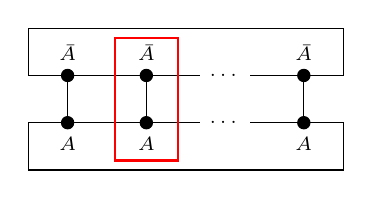
\begin{tikzpicture}[font=\scriptsize, baseline = 0.4mm, yscale=0.6]
    \draw (-0.5,0) rectangle (3.5,-1);
    \draw (-0.5,1) rectangle (3.5,2);
    \foreach \x in {0, 1, 3}{
      \node[tensor] (t) at (\x,0) {};
      \node[tensor] (s) at (\x,1) {};
      \node[anchor=north] at (\x,-0.1) {$A$};
      \node[anchor=south] at (\x,1.1) {$\bar{A}$};
      \draw (t)--(s);
    }
    \node [fill=white] at (2,0) {$\dots$};
    \node [fill=white] at (2,1) {$\dots$};
    \draw[red,thick]  (0.6,-0.8) rectangle (1.4,1.8);
  \end{tikzpicture}\ ,
\end{equation*}
where the red rectangle surrounds a copy of the transfer matrix $T$. This expression can be generalized to capture expectation values of local observables. Let us calculate the expectation value of a local observable $O$, such as  $O = X_i X_{i+1}$. As the MPS is translation invariant, we can assume w.l.o.g.\ that $O$ acts on the first few particles. 

\begin{theorem}
  Let $V$ be a vector space, and $\mathcal{H}$ be a Hilbert space. Let $A\in \End(V)\otimes \mathcal{H}$ be an MPS tensor and $T$ be its transfer matrix. Let $O\in \mathcal{B}(\mathcal{H})^{\otimes n}$ be an $m$-local observable acting on the first $m$ particles, $O = o \otimes \id^{\otimes (n-m)}$. Then
  \begin{equation*}
    \bra{\mathfrak{M}_n(A)} O \ket{\mathfrak{M}_n(A)} = \tr (T_o \cdot T^{n-m}), 
  \end{equation*}
  where 
  \begin{equation*}
    T_o = \sum_{ij} o_{i_1 \dots i_m, j_1 \dots j_m} \cdot \bar{A}_{i_1} \dots \bar{A}_{i_m} \otimes A_{j_1} \dots A_{j_m}. 
  \end{equation*}
\end{theorem}

\begin{proof}
  Direct calculation. 
\end{proof}
The graphical notation lets us visualize this calculation very succintly. For that, note that a local observable $O$ (acting on two particles) can be depicted as 
\begin{equation*}
  O = 
  \begin{tikzpicture}[baseline=4mm]
    \foreach \x in {0,1,2,4}{
      \draw (\x,0)--(\x,1);
    }
    \draw[fill=white]  (-0.2,0.4) rectangle (1.2,0.6);
    \node[fill=white] at (3,0.5) {$\dots$};
  \end{tikzpicture} \ .
\end{equation*}
Then the expecation value is depicted as 
\begin{equation*}
  \bra{\mathfrak{M}_n(A)} O \ket{\mathfrak{M}_n(A)} = 
  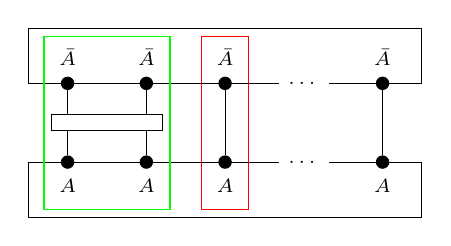
\begin{tikzpicture}[font=\scriptsize, baseline = 4mm]
    \draw (-0.5,0) rectangle (4.5,-0.7);
    \draw (-0.5,1) rectangle (4.5,1.7);
    \foreach \x in {0,1,2,4}{
      \node[tensor] (t) at (\x,0) {};
      \node[tensor] (s) at (\x,1) {};
      \node[anchor=north] at (\x,-0.1) {$A$};
      \node[anchor=south] at (\x,1.1) {$\bar{A}$};
      \draw (t)--(s);
    }
    \draw[fill=white]  (-0.2,0.4) rectangle (1.2,0.6);
    \node [fill=white] at (3,0) {$\dots$};
    \node [fill=white] at (3,1) {$\dots$};
    \draw[green]  (-0.3,-0.6) rectangle (1.3,1.6);
    \draw[red]  (2-0.3,-0.6) rectangle (2.3,1.6);
  \end{tikzpicture} \ .
\end{equation*}
The green and red rectangles denote $T_o$ and $T$, respectively. 








The transfer matrix can be viewed as the matrix representing the \emph{transfer operator} defined by
\begin{definition}[Transfer operator]
  Let $V$ be a vector space, and $\mathcal{H}$ be a Hilbert space with basis $\{\ket{i}\}_{i\in \mathcal{B}}$. Let $A\in \End(V)\otimes \mathcal{H}$ be an MPS tensor, $A = \sum_i A_i \otimes \ket{i}$. The \emph{transfer operator} of $A$ is a linear map $T: \End(V) \to \End(V)$ given by 
\begin{equation*}
  \mathbf{T}: \rho \mapsto \sum_i A_i \rho A_i^\dagger.
\end{equation*}
\end{definition}
We can actually modify our calculation such that the transfer operator appears explicitly. For that, notice that $\tr(X) = \tr(X^T)$, and thus  
\begin{equation*}
  \| \mathfrak{M}_n(A) \|^2 = \sum_{i} \tr(A_{i_1} \dots A_{i_n}) \tr (\bar{A}_{i_1} \dots \bar{A}_{j_n}) = \sum_{i} \tr(A_{i_1} \dots A_{i_n}) \tr (A^\dagger_{i_n} \dots A^\dagger_{i_1}),
\end{equation*}
Expanding the definition of the trace, we obtain
\begin{equation*}
  \| \mathfrak{M}_n(A) \|^2 = \sum_{ijk} \bra{j}A_{i_1} \dots A_{i_n}\ket{j}\bra{k} A^\dagger_{i_n} \dots A^\dagger_{i_1}\ket{k} = \sum_{jk} \bra{j} \mathbf{T}^n(\ket{j}\bra{k}) \ket{k} = \tr \mathbf{T}^n,
\end{equation*}
where we have used that the trace of a linear operator acting on matrices is calculated through $\tr X = \sum_{jk} \bra{j} X(\ket{j}\bra{k}) \ket{k}$. Similarly, expectation value of an $m$-local observable $O = o \otimes \id^{n-m}$ can be expressed as 
\begin{equation*}
  \bra{\mathfrak{M}_n(A)} O \ket{\mathfrak{M}_n(A)} =  \tr \mathbf{T}_o \mathbf{T}^{n-m},
\end{equation*}
where 
\begin{equation*}
  \mathbf{T}_o(X) = \sum_{ij} o_{i_1 \dots i_n, j_1 \dots j_n} \cdot A_{j_1} \dots A_{j_n} X A_{i_n}^\dagger \dots A_{i_1}^\dagger. 
\end{equation*}
These expressions are both very similar to the previous expressions. In fact, the matrix $T$ is just the matrix representing the linear operator $\mathbf{T}$, and $T_o$ is the matrix representing the linear operator $\mathbf{T}_o$, both written in the basis $E_{ij} = \ket{i}\bra{j}$. In particulare , $T$ and $\mathbf{T}$ has the same spectrum.  In any case, the trace of a linear map can be expressed with its eigenvalues (see \cref{fact:trace_eigen}), and thus 
\begin{equation*}
    \|\mathfrak{M}_n(A)\|^2 = \sum_{\lambda\in \mathrm{Spec}(T)} m_\lambda \cdot \lambda^n,
\end{equation*}
where $m_\lambda$ is the multiplicity of the eigenvalue $\lambda$. Note that $\mathbf{T}$ is not necessarily self-adjoint (what is the adjoint of $\mathbf{T}$?), and thus it might have complex eigenvalues. We will see, however, that $\mathbf{T}$ is a CP map, and that we can understand its spectrum as well as its fixed points; this, in fact, helps us to understand the expectation values of local observables for large system sizes (as well as in the thermodynamic limit). The (set of) theorem(s) characterizing the spectral properties of transfer operators is called Perron-Frobenius theorem. 

\subsection{The Perron-Frobenius theorem}

A short reminder:
\begin{definition}
  Let $V$ be a Hilbert space, and $X\in \End(V)$. We say that $X$ is positive if there is a finite set $ I\subset\End(V)$ such that $X = \sum_{Y\in I} Y^\dagger Y$. We say that $X$ is strictly positive if it is positive and invertible. We write $X\geq 0$ if $X$ is positive and $X>0$ if $X$ is strictly positive.
\end{definition}  
Positivity gives rise to a partial order on the set of matrices: $X\geq Y$ if and only if $X-Y\geq 0$. We also define positivity of linear maps that map matrices to matrices:

\begin{definition}  
   A linear map $\mathbf{T}:\End(V)\to \End(V)$ is called positive if $\mathbf{T}(X)\geq 0$ for all $X\geq 0$.  
\end{definition}
Let us remark that $\End(V)$ has a natural scalar product (the Hilbert-Schmidt scalar product: $\scalprod{X}{Y} = \tr\{X^\dagger Y\}$), and thus positivity on $\End(\End(V))$, i.e., on the space of $\End(V)\to \End(V)$ linear operators, could be defined analogously to how we define positivity on $\End(V)$. Our notion of positivity is different from this -- actually, a better name for it would be positivity preserving. 
\begin{exercise}
  Show that the transfer operator is positive, i.e., that $\sum_i A_i X A_i^\dagger\geq 0$ for all $X\geq 0$. 
\end{exercise}
Note that a positive map is not necessarily self-adjoint w.r.t.\ the Hilbert-Schimdt scalar product. In particular,
\begin{exercise}
  Show that the adjoint of the map $\mathbf{T}:X\mapsto \sum_i A_i X A_i^\dagger$ is the map $\mathbf{T}^\dagger:X\mapsto \sum_i A_i^\dagger X A_i$.
\end{exercise}
Be aware of the notation here: $\mathbf{T}(X)^\dagger \neq \mathbf{T}^\dagger(X)$. Instead, as $\mathbf{T}$ is positivity preserving, it commutes with the dagger operation, $\mathbf{T}(X)^\dagger = \mathbf{T}(X^\dagger)$. The transfer operator actually has a stronger property than positivity, complete positivity:
\begin{definition}[Complete positivity]
  Let $V$ be a vector spaces, $\mathbf{T}:\End(V) \to \End(V)$ be a linear map. We say that $\mathbf{T}$ is completely positive if for all $d\in\mathbb{N}^+$ the map $\mathbf{T}\otimes \id: \End(V)\otimes \mathcal{M}_d \to \End(V)\otimes \mathcal{M}_d $ is positive. 
\end{definition}
\begin{exercise}
  Show that the transfer operator is completely positive. 
\end{exercise}


We have seen that MPS for which there is a non-trivial projector $P$ such that $A_iP = PA_iP$ can be written as a sum of two smaller bond dimensional translation invariant MPS. 
\begin{exercise}
  Show that if there is a non-trivial projector $P$ such that $A_iP = PA_iP$, then there is also such a non-trivial \emph{orthogonal} projector $P$. (Hint: both conditions are equivalent to finding a subspace invariant under all MPS matrices.)
\end{exercise}
This property is reflected in the transfer matrix of the MPS:
\begin{theorem}
  Let $V$ be a vector space, and $\mathcal{H}$ be a Hilbert space with basis $\{\ket{i}\}_{i\in \mathcal{B}}$. Let $A\in \End(V)\otimes \mathcal{H}$ be an MPS tensor, $A = \sum_i A_i \otimes \ket{i}$. Let $P$ be an orthogonal projector and let $\mathbf{T}$ be the transfer operator of the MPS. Then the following are equivalent:
  \begin{enumerate}
    \item  $A_i P = P A_i P$ for all $i\in \mathcal{B}$,
    \item there is $\lambda\in \mathbb{R}^+$ such that $\mathbf{T}(P)\leq \lambda P$.
  \end{enumerate}
  If there is such a non-trivial ($P\neq 0, \ \id$) orthogonal projector, then the transfer operator of the MPS is called \emph{reducible}. Otherwise it is called \emph{irreducible}.
\end{theorem}

\begin{proof}
  Let us first show $1\Rightarrow 2$: assume that $A_i P = P A_i P$. Then
  \begin{equation*}
    \mathbf{T}(P) = \sum_i A_i P A_i^\dagger = \sum_i PA_iPA_i^\dagger P = P\mathbf{T}(P)P \leq  \|\mathbf{T}(P)\| \cdot P.
  \end{equation*}
  Let us now show $2\Rightarrow 1$: for that, let us note that if $\mathbf{T}(P)\leq \lambda P$, then $(1-P) \mathbf{T}(P) (1-P) \leq \lambda (1-P)P(1-P) = 0$, and thus $(1-P) \mathbf{T}(P) (1-P) = 0$. Then
  \begin{equation*}
    0 = (1-P)\mathbf{T}(P)(1-P) = \sum_i (1-P)A_i P A_i^\dagger (1-P).
  \end{equation*} 
  The last expression is a sum of positive operators, and thus it can be $0$ only if all the summands are $0$, i.e., $(1-P)A_i P A_i^\dagger (1-P) = 0$  for all $i$, or equivalently, $(1-P)A_i P =0$. 
\end{proof}

Before stating the Perron-Frobenius theorem, we need the following lemma:
\begin{lemma}\label{lem:irreducible_invertibility}
  Let $\mathbf{T}$ be an irreducible CP map. Then there is $n\in \mathbb{N}^+$ such that $(1+\mathbf{T})^n(X) > 0$ (i.e., strictly positive) for all $X\geq 0$, $X\neq 0$.
\end{lemma}

\begin{proof}
  Let $X\geq 0$, $X\neq 0$. Then, as $\mathbf{T}(X)$ is positive, the kernel of $(1+\mathbf{T})(X) = X+\mathbf{T}(X)$ is contained in the kernel of $X$: for $v\in \ker(X + \mathbf{T}(X))$,
  \begin{equation*}
    0 = \bra{v} X + \mathbf{T}(X) \ket{v} = \bra{v} X \ket{v} +  \bra{v} \mathbf{T}(X) \ket{v};
  \end{equation*}
  As both summands are non-negative, both of them are $0$, and in particular, $\bra{v} X \ket{v} = 0$, i.e., $v\in\ker(X)$. We thus obtained that $\ker(X)\geq \ker((1+\mathbf{T})(X)) \geq \dots \geq \ker((1+\mathbf{T})^n (X))$. As the dimension of these spaces is non-increasing, we can find $n$ such that $\ker (Y) = \ker(Y + \mathbf{T}(Y))$ for  $Y = (1+\mathbf{T})^n(X)\neq 0$. 
  Let $P$ be the projector onto the range of $Y$, such that $ P \leq \lambda Y$ for some $\lambda\in\mathbb{R}^+$. As $\ker (Y) = \ker(Y + \mathbf{T}(Y))$, their range is the same as well, and thus there is $\mu\in\mathbb{R}^+$ such that $Y + \mathbf{T}(Y) \leq \mu P$. Then
  \begin{equation*}
    \mathbf{T}(P) \leq \lambda \mathbf{T}(Y) \leq \lambda(Y+\mathbf{T}(Y)) \leq \lambda\mu P,
  \end{equation*}
  and thus by irreducibility of $\mathbf{T}$, $P=0$ or $P=1$. As $X\neq 0$, $Y\neq 0$ neither, and thus  $P = 1$, i.e., $Y = (1+\mathbf{T})^n(X)$ is invertible.
\end{proof}

We now arrive at the core argument of the Perron-Frobenius theorem:
\begin{theorem}
  Let $\mathbf{T}$ be an irreducible CP map on a finite dimensional Hilbert space $V$. Then the following expression is finite: 
  \begin{equation*}
  \lambda = \sup_{X\geq 0} \sup \{\rho\in \mathbb{R}_+| \rho X \leq \mathbf{T}(X) \}.
  \end{equation*} 
  Moreover, $\lambda$ is a simple eigenvalue of $\mathbf{T}$ with a strictly positive eigenvector $X$.
\end{theorem}

We will call $\lambda$ the characteristic eigenvalue and $X$ (unique up to a multiplicative constant) the characteristic eigenvector of $\mathbf{T}$.

\begin{proof}
  Let $r(X) = \sup \{\rho\in \mathbb{R}_+| \rho X \leq \mathbf{T}(X) \}$ be defined on positive matrices. We will show that $r(X)$ attains its maximum on a strictly positive $X$, and that $\mathbf{T}(X) = r(X)\cdot X$, i.e.\ that $r(X)$ is the characteristic eigenvalue and $X$ is the characteristic eigenvector of  $\mathbf{T}$.  
  
  We will try to reduce the problem of finding the maximum of $r$ to maximizing a continuous function on a compact region. The function $r$, however, is, in general, not continuous and it is defined on an unbounded set. Let us show thus that there is a compact set $S$ where $r$ is continuous and where $\forall Y\notin S$ there is $X\in S$ such that $r(X)\geq r(Y)$. 
  
  The first insight into constructing $S$ is that $r$ is continuous on invertible matrices. To see this, note first that due to irreducibility of $\mathbf{T}$, if $\mathbf{T}(1)\leq \mu P$ for a projector $P$ and $\mu\in \mathbb{R}^+$, then $\mathbf{T}(P)\leq \mathbf{T}(1) \leq \mu P$, and thus $P=1$. This implies that $\mathbf{T}(1)$ is invertible. Therefore if $X>0$, then there is $\nu>0$ such that $\nu 1 \leq X$, and thus $ \nu \mathbf{T}(1)\leq \mathbf{T}(X)$, i.e., $\mathbf{T}(X)$ is invertible as well. We can thus write $r(X)^{-1} = \|\mathbf{T}(X)^{-1/2}X \mathbf{T}(X)^{-1/2}\|$, which is continuous.
  
  Secondly, note that $r(\mu X) = r(X)$ for any $\mu\in\mathbb{R}^+$, and thus we can try to maximize $r$ on the compact set $R = \{ X\geq 0 \text{ and } \|X\|\leq 1\}$. Finally note that due to \cref{lem:irreducible_invertibility} there is $n$ such that all matrices in the compact set $S = (1+\mathbf{T})^n(R)$ are invertible. Let us show that we can maximize $\mathbf{T}$ on the set $S$: given $X\in R$, we have $\mathbf{T}(X) - r(X) X\geq 0$. We can apply $(1+\mathbf{T})^n$ on this matrix and obtain either $\mathbf{T}(X) = r(X) X$, or $0 < (1+\mathbf{T})^n(X) = \mathbf{T}(Y)- r(X) Y$, where $Y = (1+\mathbf{T})^n(X)$. As $\mathbf{T}(Y)- r(X) Y> 0$, this implies that 
  \begin{equation}\label{eq:r_maximum_constraint}
    r(Y) \geq r(X) \text{ with $Y = (1+\mathbf{T})^n(X)$, and equality holds only if  $\mathbf{T}(X) = r(X) X$}.
  \end{equation}
  Therefore we can maximize $\mathbf{T}$ on the image of $(1+\mathbf{T})^n$. This is a compact set consisting of invertible matrices and thus $r$ is continuous on it. Thus $r$ attains its maximum and it is on a strictly positive (invertible) matrix $X$. In this maximum equality holds in \cref{eq:r_maximum_constraint}, and thus $X$ is an eigenvalue with $\lambda:=r(X)$.
  
  Let us show now that $X$ is the unique eigenvector of $\lambda$. Assume that $Y$ is another eigenvector for $\lambda$. Then, as $\lambda$ is real, $Y^*$ is also an eigenvector with $\lambda$, and thus the self-adjoint operators $Y+Y^*$ and $i(Y-Y^*)$ are eigenvectors as well. We can thus assume w.l.o.g.\ that $Y$ is self-adjoint. As $X$ is invertible, we can find $\mu\in \mathbb{R}^+$ such that $\mu X-Y \geq 0$, but it is not strictly positive. If $\mu X-Y\neq 0$, then $(1+\lambda)^n(\mu X - Y) = (1+\mathbf{T})^n(\mu X - Y)> 0$, contrary to the assumption, thus $\mu X = Y \geq 0$. We have thus obtained that $X$ is the unique eigenvector for $\lambda$.
\end{proof}




We will show now that the characteristic eigenvalue of an irreducible CP map $\mathbf{T}$ is its spectral radius. For that, we need more tools: namely, that CP maps satisfy a suitable generalization of the Cauch-Schwartz inequality. It is easiest to state it for CP maps that leave $1$ invariant (also called unital):
\begin{lemma}[Schwarz inequality]\label{lem:Schwarz}
  Let $\mathbf{T}:\End(V) \to \End(V)$ be a completely positive map such that $\mathbf{T}(1)=1$. Then 
  \begin{equation*}
    \mathbf{T}(x) \mathbf{T}(x)^* \leq \mathbf{T}(xx^*) \quad \forall x\in\End(V).
  \end{equation*}
  Moreover, if equality holds for some $x\in\End(V)$, then 
  \begin{equation*}
    \mathbf{T}(x) \mathbf{T}(y) = \mathbf{T}(xy)  \quad \forall y\in\End(V).
  \end{equation*}
\end{lemma}
\begin{proof}
  If $\mathbf{T}$ is completely positive, then it is also $2$-positive: $\mathbf{T}\otimes \id_2$ maps positive matrices to positive matrices. Let us consider the matrix 
  \begin{equation*}
   M = \left(\begin{matrix} 1 & x^* \\ x & xx^* \end{matrix}\right)
  \end{equation*}
  $M$ is positive, as 
  \begin{equation*}
   M = \left(\begin{matrix} 1 & x^* \\ x & xx^* \end{matrix}\right)
   = \left(\begin{matrix} 1  \\ x \end{matrix}\right) \cdot \left(\begin{matrix} 1 & x^*  \end{matrix}\right). 
  \end{equation*}
  Positivity of $\mathbf{T}\otimes \id_2$ implies then that 
  \begin{equation*}
   (\mathbf{T}\otimes\id)(M) = \left(\begin{matrix} 1 & \mathbf{T}(x^*) \\ \mathbf{T}(x) & \mathbf{T}(xx^*) \end{matrix}\right) \geq 0, 
  \end{equation*}
  where we have used $\mathbf{T}(1)=1$. Then the following matrix is also positive:
  \begin{equation*}
   0 \leq \left(\begin{matrix} -\mathbf{T}(x) & 1 \end{matrix}\right) \cdot
          \left(\begin{matrix} 1 & \mathbf{T}(x^*) \\ \mathbf{T}(x) & \mathbf{T}(xx^*) \end{matrix}\right) \cdot
          \left(\begin{matrix} -\mathbf{T}(x^*) \\ 1 \end{matrix}\right) = \mathbf{T}(xx^*) - \mathbf{T}(x)\mathbf{T}(x^*),
  \end{equation*}
  which is the desired inequality.
  
  Assume now that $x$ is such that $\mathbf{T}(x) \mathbf{T}(x)^* = \mathbf{T}(xx^*)$. Consider then the Schwarz inequality for $\lambda x +y$ for some $\lambda\in\mathbb{R}$: 
  \begin{equation*}
    \lambda^2 \mathbf{T}(x)\mathbf{T}(x^*) + \lambda \mathbf{T}(x) \mathbf{T}(y^*) + \lambda \mathbf{T}(y^*) \mathbf{T}(x) + \mathbf{T}(y)\mathbf{T}(y^*)\leq \lambda^2 \mathbf{T}(xx^*) + \lambda  \mathbf{T}(xy^*)  + \lambda \mathbf{T}(yx^*) + \mathbf{T}(yy^*).
  \end{equation*} 
  The second order terms cancel, thus we obtain
  \begin{equation*}
     0 \leq \lambda [ \mathbf{T}(xy^*) +  \mathbf{T}(yx^*) - \mathbf{T}(x) \mathbf{T}(y^*) -  \mathbf{T}(y^*) \mathbf{T}(x)]  + \mathbf{T}(yy^*) - \mathbf{T}(y)\mathbf{T}(y^*).
  \end{equation*} 
  As this holds for all $\lambda\in\mathbb{R}$, 
  \begin{equation*}
  \mathbf{T}(xy^*) +  \mathbf{T}(yx^*) - \mathbf{T}(x) \mathbf{T}(y^*) -  \mathbf{T}(y) \mathbf{T}(x^*) = 0.
  \end{equation*}
  Notice now that if $x$ satisfies equality in the Schwarz inequality, then $ix$ also satisfies equality. We thus obtain that 
  \begin{equation*}
    i \mathbf{T}(xy^*) -i \mathbf{T}(yx^*) - i \mathbf{T}(x) \mathbf{T}(y^*)  + i  \mathbf{T}(y) \mathbf{T}(x^*) = 0,
  \end{equation*}
  as well. A linear combination of these two equations yield $\mathbf{T}(xy^*) = \mathbf{T}(x) \mathbf{T}(y)^*$. 
\end{proof}


We can now state and prove the Perron-Frobenius theorem for CP maps that are \emph{irreducible}. 
\begin{theorem}
  Let $\mathbf{T}:\End(V)\to\End(V)$ be a CP map, where $V$ is a finite dimensional Hilbert space. Then 
  \begin{itemize}
  \item  $\exists \lambda\in \mathrm{Spec}(\mathbf{T})\cap \mathbb{R}^+$ such that for all $\mu\in \mathrm{Spec}(\mathbf{T})$, $|\mu|\leq \lambda$. 
  \item  There is a strictly positive eigenvector with eigenvalue $\lambda$. 
  \item If $\mu\in \mathrm{Spec}(\mathbf{T})$ is such that $|\mu| =  \lambda$, then $\mu = \epsilon \cdot \lambda$ with $\epsilon^{\dim(V)^2} =1 $.
  \end{itemize}
\end{theorem}

\begin{proof}
  Let $\lambda$ be the characteristic eigenvalue of $\mathbf{T}$ with the strictly positive eigenvector $X$. We will show now that $\lambda$ is the largest eigenvalue. Let us define the map 
  \begin{equation*}
    S: Z \mapsto \lambda^{-1} \cdot X^{-1/2}\mathbf{T}(X^{1/2} Z X^{1/2}) X^{-1/2}.
  \end{equation*}
  It is straightforward to verify that $S$ is CP, and that its characteristic eigenvalue is $1$ with characteristic eigenvector $\id$. Moreover, $Y$ is an eigenvector of $\mathbf{T}$ with eigenvalue $\mu$ if and only if $Z = X^{-1/2} Y X^{-1/2}$ is an eigenvector of $S$ with eigenvalue $\mu/\lambda$. Let $Z$ be such an eigenvector of $S$. Then, through the Schwarz inequality,
  \begin{equation*}
    |\mu/\lambda|^2 Z Z^* = S(Z) S(Z^*) \leq S(ZZ^*).
  \end{equation*}
  By definition of the characteristic eigenvalue (that is, $\sup_{W\geq 0}\sup\{\rho\in \mathbb{R}^+ | \rho W \leq S (W)\} = 1$), this implies that $|\mu|\leq |\lambda|$, i.e.\ $\lambda$ is the largest eigenvalue of $\mathbf{T}$. Moreover, if $|\mu| = |\lambda|$, then equality holds in the Schwarz inequality, and thus, if $W$ is another eigenvalue of $S$ with $\nu$ such that $|\nu|=1$, then 
  \begin{equation*}
    \nu \mu/ \lambda \cdot ZW = S(Z) S(W)  =  S(ZW),
  \end{equation*}
  therefore $ZW$ is also an eigenvector of $S$, with eigenvalue $\nu\mu/\lambda$. Therefore the eigenvalues on the periphery of the spectrum of $S$ form a group. As there is at most $\dim(V)^2$ of these eigenvalues, they are powers of $\dim(V)^2$-th unit roots. Consequently any eigenvalue on the periphery of the spectrum of $\mathbf{T}$ can be written as $\epsilon\cdot \lambda$, where $\epsilon$ is a $\dim(V)^2$-th unit root.
\end{proof}


\begin{remark}
  If $\mathbf{T}$ has eigenvalues on the periphery of the spectrum, then, as it is a root of unity, there is $n$ such that the largest eigenvalue of $\mathbf{T}^n$ is degenerate. This implies that $\mathbf{T}^n$ is reducible. 
\end{remark}

Finally, for general MPS tensors (not necessarily injective, and might even be reducible without blocking) these results generalize the  following way:
\begin{theorem}
  Let $\mathbf{T}$ be a CP map on a finite dimensional Hilbert space $V$. Then 
  \begin{itemize}
  \item  $\exists \lambda\in \mathrm{Spec}(\mathbf{T})\cap \mathbb{R}^+$ such that for all $\mu\in \mathrm{Spec}(\mathbf{T})$, $|\mu|\leq \lambda$. 
  \item  There is a positive (but not necessarily strictly positive) eigenvector with eigenvalue $\lambda$. 
  \end{itemize}
\end{theorem}
\begin{proof}
  Let us fix an irreducible CP map $S$, and consider the map $\mathbf{T}_n = \mathbf{T}+\tfrac{1}{n}S$. This map is also irreducible and $\mathbf{T}_n \to \mathbf{T}$ as $n\to \infty$. Let $X_n$ be the characteristic eigenvalue of $\mathbf{T}_n$ with eigenvalue $\lambda_n$. Then $X_n\to X$, a positive (but not necessarily invertible) element and $\mathbf{T}(X) = \lambda X$. Moreover, $\lambda$ is the spectral radius of $\mathbf{T}$. 
\end{proof}


\paragraph{Example.} Let us consider the state $\ket{0}^{\otimes n} + \lambda^n \cdot \ket{1}^{\otimes n}$, with $|\lambda|\leq 1$. This state can be written as an MPS with tensors 
\begin{equation*}
  A_0 = \left(\begin{matrix}
    1 & 0 \\ 0 & 0 
  \end{matrix}\right), \quad 
  A_1 = \left(\begin{matrix}
    0 & 0 \\ 0 & \lambda 
  \end{matrix}\right).
\end{equation*}
The corresponding transfer operator acts as 
\begin{equation*}
  \mathbf{T}: \rho \mapsto \bra{0}\rho\ket{0} \cdot \ket{0}\bra{0} + |\lambda |^2 \bra{1}\rho\ket{1} \cdot \ket{1}\bra{1}.
\end{equation*}
This map has three eigenvalues: $0,|\lambda|$, and $1$. The spectral radius of $\mathbf{T}$ is 1; this is an eigenvalue of $\mathbf{T}$. If $|\lambda|<1$, then the eigenvalue $1$ is simple, and the corresponding eigenvector, $\ket{1}\bra{1}$, is positive, but not invertible. If $|\lambda|=1$, the eigenvalue $1$ is degenerate: the corresponding eigenspace is two dimensional spanned by $\ket{0}\bra{0}$ and $\ket{1}\bra{1}$. Notice that this space contains strictly positive eigenvectors, e.g., $\id>0$.

\subsection{Application of the Perron-Frobenius theorem}
Let us consider an MPS tensor $A$. Assume that $A$ is such that there is no projector $P$ for any $n$ such that $A_{i_1} \dots A_{i_n} P = PA_{i_1} \dots A_n P$. Then its transfer matrix is irreducible and it has no peripheral spectrum (i.e.\ all other eigenvalues have absolute values strictly smaller than the spectral radius), and thus we can write $\mathbf{T}$ as 
\begin{equation*}
  \sum_{\mu\in \mathrm{Spec}(\mathbf{T})} \mu P_{\mu} + N = \lambda \ket{L}\bra{R} + \sum_{|\mu|<\lambda} \mu P_\mu + N,
\end{equation*} 
where $P_\mu$ is a projector and $N$ is a nilpotent matrix commuting with all $P_\mu$. We have used that $\lambda$ is a simple eigenvector and thus $P_\lambda = \ket{L}\bra{R}$ for some $L,R$ matrices (here the bra-ket notation is the following: the ket denotes matrices, the bra linear functionals of the form $\scalprod{R}{X} = \tr\{R^\dagger X\}$). $L$ is the fixed point of $T$, while $R$ is the fixed point of $T^\dagger$. They are both strictly positive matrices. As $N$ commutes with $\ket{L}\bra{R}$, $N\ket{L} \bra{R} = \ket{L}\bra{R}N$, $L$ and $R$ are left- and right eigenvectors of $N$. But as $N$ is nilpotent, the corresponding eigenvalue has to be zero, and thus $N\ket{L} = 0$ and $\bra{R}N = 0$. Let the rank of $N$ be $k$, $N^{k+1} = 0$. 

We can now calculate $T^n$:
\begin{equation*}
  T^n = \lambda^n \ket{L}\bra{R} + \sum_{m=0}^{k} { n \choose m} \mu^{n-m} P_\mu N^m, 
\end{equation*} 
and thus
\begin{equation*}
  \| \lambda^{-n}T^n - \ket{L}\bra{R} \|  \leq \sum_{m=0}^{k} { n \choose m} |\mu/\lambda|^{n-m} \|N^m\|\leq c \cdot \nu^n, 
\end{equation*} 
where $c$ is a sufficiently large constant and $0<\nu<1$. This means that $\lambda^{-n}T^n$ converges exponentially to $\ket{L}\bra{R}$. Graphically,
\begin{equation*}
  \lambda^{-n}T^n = \lambda^{-n}
  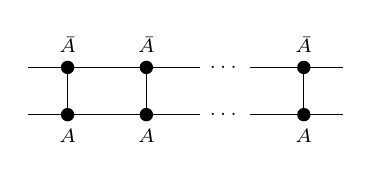
\begin{tikzpicture}[font=\scriptsize, baseline = 2mm, yscale=0.6]
    \draw (-0.5,0) -- (3.5,0);
    \draw (-0.5,1) -- (3.5,1);
    \foreach \x in {0, 1, 3}{
      \node[tensor] (t) at (\x,0) {};
      \node[tensor] (s) at (\x,1) {};
      \node[anchor=north] at (\x,-0.1) {$A$};
      \node[anchor=south] at (\x,1.1) {$\bar{A}$};
      \draw (t)--(s);
    }
    \node [fill=white] at (2,0) {$\dots$};
    \node [fill=white] at (2,1) {$\dots$};
  \end{tikzpicture} \rightarrow
  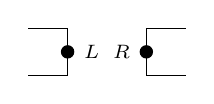
\begin{tikzpicture}[font=\scriptsize, baseline = -1mm, yscale=0.3]
    \draw (-0.5,1) -- (0,1) -- (0,-1) -- (-0.5,-1);
    \node[tensor,label=east:$L$] at (0,0) {};
    \draw (1.5,1) -- (1,1) -- (1,-1) -- (1.5,-1);
    \node[tensor,label=west:$R$] at (1,0) {};
  \end{tikzpicture}.
\end{equation*}
As the map 
\begin{equation*}
  X \mapsto 
  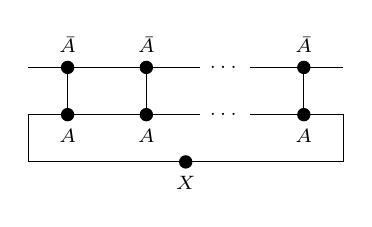
\begin{tikzpicture}[font=\scriptsize, baseline = 0.4mm, yscale=0.6]
    \draw (-0.5,0) rectangle (3.5,-1);
    \draw (-0.5,1) -- (3.5,1);
    \node[tensor] (t) at (1.5,-1) {};
    \node[anchor=north] at (1.5,-1.1) {$X$};
    \foreach \x in {0, 1, 3}{
      \node[tensor] (t) at (\x,0) {};
      \node[tensor] (s) at (\x,1) {};
      \node[anchor=north] at (\x,-0.1) {$A$};
      \node[anchor=south] at (\x,1.1) {$\bar{A}$};
      \draw (t)--(s);
    }
    \node [fill=white] at (2,0) {$\dots$};
    \node [fill=white] at (2,1) {$\dots$};
  \end{tikzpicture}\   \xrightarrow[n\to \infty]{} LXR, 
\end{equation*}
and both $L$ and $R$ are invertible, the limit is invertible, and thus there is $N$ such that it is invertible $\forall n> N$. In particular, for such an $n$, the MPS $\mathfrak{M}_n(A,X)$ is non-zero if $X$ is not $0$. Equivalently, the MPS defined by the tensor $A$ is injective. We have thus proven \cref{thm:MPS_decomposition}: if the MPS matrix is not reducible nor does it become reducible after blocking enough matrices, then it is injective.


Let us consider now the overlap of two MPS. We can write
\begin{equation*}
  \frac{|\scalprod{\mathfrak{M}_n(A)}{\mathfrak{M}_n(B)}|^2}{\|\mathfrak{M}_n(A)\|\cdot\|\mathfrak{M}_n(B)\|} = \frac{|\tr T_{AB}^n|^2}{\tr T_A^n \tr T_B^n} \leq 1,
\end{equation*}
where $T_{AB}$ is the mixed transfer matrix, with corresponding transfer operator $\mathbf{T}_{AB}(X) = \sum_i A_i X B_i^\dagger$ (it is not a CP map). The dominating term in the denominator is $\lambda_A^n\lambda_B^n$, and thus the absolute value of the largest eigenvalue of $T_{AB}$ is at most $\lambda_A \lambda_B$. If it is smaller than $\lambda_A\lambda_B$, the overlap tends to zero as $n\to \infty$. To examine the case where the absolute value of the largest eigenvalue of $T_{AB}$ is $\lambda_A \lambda_B$, we will use a Cauchy-Schwarz inequality. Let us assume $X$ is an eigenvector of $T_{AB}$ with eigenvalue $\mu$ and $\rho$ is the characteristic eigenvector of $T_A$, then 
\begin{equation*}
  \left|\mu \cdot \tr(X^\dagger\rho X)\right|^2 = |\tr(X^\dagger \rho T_{AB}(X) )|^2 = \left|\sum_i \tr(X^\dagger \rho  A_i X B_i^\dagger )\right|^2 = \left|\sum_i \tr(\underbrace{B_i^\dagger  X^\dagger \rho^{1/2}}\underbrace{\rho^{1/2}  A_i X} )\right|^2.
\end{equation*}
Using now the Cauchy-Schwarz inequality for the expression above, we obtain
\begin{equation*}
  \left|\mu \cdot \tr(X^\dagger\rho X)\right|^2  \leq \sum_i \tr(B_i^\dagger X^\dagger \rho X B_i) \cdot \sum_i \tr(X^\dagger A_i^\dagger \rho A_i X) \leq \lambda_A\lambda_B \left(\tr(X^\dagger \rho X)\right)^2,
\end{equation*}
where we have used that $\rho$ is an eigenvector of $T_A$ with eigenvalue $\lambda_A$, and, as $\lambda_B$ is the characteristic eigenvalue of $T_B$ and $X^\dagger \rho X\geq 0$, that $T_B(X^\dagger \rho X)\leq \lambda_B X^\dagger \rho X$. Notice now that $\tr(X^\dagger \rho X) \neq 0$ if $X\neq 0$, and thus $\mu \leq \lambda_A\lambda_B$, and if equality holds, then (1) there is $\alpha\in\mathbb{C}$, $|\alpha|=1$,  such that $\rho^{1/2} X B_i = \alpha \rho^{1/2} A_i X$ for all $i$, and (2) $X^\dagger \rho X$ is the characteristic eigenvector of $T_B$. Because of (2), $X$ is invertible and thus (1) is equivalent with $B_i = \alpha X^{-1} A_i X$. We have thus learned that 
\begin{theorem}
  Let $A$ and $B$ be two injective MPS tensors. Then either they are orthogonal in the thermodynamic limit,
  \begin{equation*}
   \frac{|\scalprod{\mathfrak{M}_n(A)}{\mathfrak{M}_n(B)}|^2}{\|\mathfrak{M}_n(A)\|\cdot\|\mathfrak{M}_n(B)\|} \rightarrow_{n\to\infty} 0,
  \end{equation*} 
  or they generate the same state (up to a phase), and in fact, they are related with an inertible $X$ and $\alpha\in \mathbb{C}$, $|\alpha|=1$ as 
  \begin{equation*}
    B_i = \alpha X^{-1} A_i X.
  \end{equation*}
\end{theorem}


\section{Parent Hamiltonians}

As solving many-body Hamiltonians can be very challenging, one at least wants to find out what are the possible ``different behaviors'' that ground states of Hamiltonians can exhibit. For that, being able to find examples of local Hamiltonians with exactly known ground states becomes important. Matrix product states make this possible: for any injective MPS, one can create a local Hamiltonian such that the MPS is its unique ground state. This construction is known as the parent Hamiltonian construction.

\paragraph{Remark.} The word \emph{local} is important: for any state $\ket{\Psi}$ the Hamiltonian $H = 1 - \ket{\Psi}\bra{\Psi}$ has $\ket{\Psi}$ as unique ground state. This Hamiltonian, however, is not local. Similarly, it is important that we want \emph{unique} ground state (or later on, ground space that is not too degenerate): the Hamiltonian $H=\id$ is local, and any state is a ground state of it -- thus it is not an interesting example.

\begin{definition}[MPS space]
  Let $V$ be a vector space and $\mathcal{H}$ be a Hilbert space with basis $\mathcal{B} = \{\ket{0},\ket{1},\dots \ket{d-1}\}$. Let $A\in \End(V)\otimes \mathcal{H}$, $A = \sum_{i\in \mathcal{B}} A_i \otimes \ket{i}$ be an MPS tensor. The MPS space on $n$ sites, $\mathfrak{S}_n(A)\subseteq \mathcal{H}^{\otimes n}$, is the collection of the open boundary MPS with all boundary conditions,
  \begin{equation*}
    \mathfrak{S}_n(A) = \left\{\mathfrak{M}_n(A,X) \middle| X\in \End(V) \right\} = \left\{\sum_{i\in \mathcal{B}^n} \tr\left\{XA_{i_1} A_{i_2} \dots A_{i_n}\right\} \ket{i_1 i_2 \dots i_n}\middle| X\in \End(V)\right\}.
  \end{equation*}
\end{definition}

Notice that if $\dim(V)=D$, then the dimension of $\mathfrak{S}_n(A)$ is at most $D^2 = \dim (\End(V))$, independent of $n$. As the size of the $n$-body Hilbert space is $d^n$, this means that there is $n$ such that $\dim(\mathfrak{S}_n(A))< \dim \mathcal{H}^{\otimes n}$, i.e,  $\mathfrak{S}_n(A)\subsetneq \mathcal{H}^{\otimes n}$.

\begin{definition}[Parent Hamiltonian]
  Let $A$ be an MPS tensor in a Hilbert space $\mathcal{H}$. Assume that $k$ is such that $\mathfrak{S}_k(A)\subsetneq \mathcal{H}^{\otimes k}$. Let $h\in \mathcal{B}(\mathcal{H})^{\otimes k}$ be the orthogonal projector onto $\mathfrak{S}_k(A)^\perp$. The $N$-body open boundary \emph{parent Hamiltonian} $H\in\mathcal{B}(\mathcal{H})^{\otimes N}$ of the MPS is 
  \begin{equation*}
    H_{OBC}^{(N)} = \sum_{i=0}^{N-k} \id^{\otimes i} \otimes h \otimes \id^{\otimes N-i-k} = \sum_{i=0}^{N-k} \tau^i(h\otimes \id^{\otimes N-k}),
  \end{equation*}
  where $\tau$ is the translation operator. The $N$-body periodic boundary parent Hamiltonian is
  \begin{equation*}
    H_{PBC}^{(N)} = \sum_{i=0}^{N-1} \tau^i(h\otimes \id^{\otimes N-k}),
  \end{equation*}
  where we index the sites $mod(N)$, that is, $\tau^k (\id^{\otimes N-1} \otimes A) = \id^{\otimes (k-1)} \otimes A \otimes id^{\otimes N-k}$, for all $A\in\mathcal{B}(\mathcal{H})$.  
\end{definition}

Any MPS is a ground state of its parent Hamiltonian: This is because the parent Hamiltonian checks whether a state ``locally looks like the MPS''. Formally, by definition,  $\mathfrak{M}_n(A,X)\in \mathfrak{S}_k \otimes \mathcal{B}(\mathcal{H})^{\otimes (n-k)}$, and thus $(h\otimes \id^{n-k}) \mathfrak{M}_n(A,X) = 0$. Similarly,  $\mathfrak{M}_n(A,X)$ is a zero-energy eigenstate of $\tau^i(h\otimes \id^{\otimes N-k})$, for any $i=0\dots n-k$, and thus it is a zero-energy eigenstate of the open boundary parent Hamiltonian $H_{OBC}^{(n)}$.  Moreover, the state $\mathfrak{M}_n(A)= \mathfrak{M}_n(A,\id)$ is also zero-energy eigenstate of $\tau^i(h\otimes \id^{\otimes n-k})$, for $i>n-k$, and thus $\mathfrak{M}_n(A)$ is a zero-energy eigenstate of the periodic boundary parent Hamiltonian $H_{PBC}^{(n)}$. Finally, as the parent Hamiltonian (both open and periodic boundary) is a sum of orthogonal projectors, it is a positive operator, and thus a zero-energy eigenstate is a ground state.

Under certain conditions we can prove that these states are the \emph{only} ground states of the Hamiltonian.  

\begin{theorem}
  Let $A\in\End(V)\otimes \mathcal{H}$ be an \emph{injective} MPS tensor with injectivity length $k-1$. Then the ground space of the $k$-body open boundary parent Hamiltonian  on $n$ sites, $H_{OBC}^{(n)}$, is $\mathfrak{S}_n(A) = \{\mathcal{M}_n(A,X)|X\in \End(V)\}$. Moreover, the ground space of the the $k$-body periodic boundary parent Hamiltonian  on $n$ sites, $H_{PBC}^{(n)}$, is $\mathbb{C} \mathfrak{M}_n(A)$. 
\end{theorem}

\begin{proof}
  First we prove the open boundary case. Let us prove by induction on $n$, starting from $k-1$. The statement, by definition of the parent Hamiltonian, is true for $k-1$. Let us assume that for $n$ the ground space of $H_{OBC}^{(n)}$ is $\mathfrak{S}_n$, we want to prove that the ground space of $H_{OBC}^{(n+1)}$ is $\mathfrak{S}_{n+1}$. We have already checked that any state from $\mathfrak{S}_{n+1}$ is a zero energy (and thus ground) state of $H_{OBC}^{(n+1)}$, we thus only have to prove that there are no other zero energy states. As $H_{OBC}^{(n+1)} = H_{OBC}^{(n)}\otimes\id + \id^{\otimes (n-1)}\otimes h \geq H_{OBC}^{(n)}\otimes \id$, and similarly, $H_{OBC}^{(n+1)}\geq \id\otimes H_{OBC}^{(n)}$, the zero energy space of $H_{OBC}^{(n+1)}$ is exactly $\mathfrak{S}_n\otimes \mathcal{H}\cap \mathcal{H} \otimes \mathfrak{S}_n$.
  We thus need to prove that  $\mathfrak{S}_{n+1}\subseteq \mathfrak{S}_n\otimes \mathcal{H}\cap \mathcal{H} \otimes \mathfrak{S}_n$. As $\mathfrak{S}_n\subseteq \mathfrak{S}_{1} \otimes \mathfrak{S}_{n-1}$ and $\mathfrak{S}_{n}\subseteq \mathfrak{S}_{n-1} \otimes \mathfrak{S}_{1}$, it is easy to see that $\mathfrak{S}_n\otimes \mathcal{H}\cap \mathcal{H} \otimes \mathfrak{S}_n = \mathfrak{S}_n\otimes \mathfrak{S}_1\cap \mathfrak{S}_1 \otimes \mathfrak{S}_n$. Let us consider now a state $\phi$ from $\mathfrak{S}_n\otimes \mathfrak{S}_1\cap \mathfrak{S}_1 \otimes \mathfrak{S}_n$. By assumption, we can write it as 
  \begin{equation*}
    \phi = \sum_i \mathfrak{M}_n(A,X_i) \otimes \mathfrak{M}_1(A,Y_i) = \sum_{ij} \tr(A_{i_1} \dots A_{i_n} U_j A_{i_{n+1}} W_j) \ket{i_1 \dots i_{n+1}},
  \end{equation*}
  where $U_j$ and $W_j$ are matrices such that $\sum_j U_j \otimes W_j = \sum_{iklrs} (X_{i})_{kl} (Y_i)_{rs} \ket{k}\bra{s} \otimes \ket{r}\bra{l}$. Similarly, as $\phi\in \mathfrak{S}_1 \otimes \mathfrak{S}_n$, there are matrices $Z_j,V_j$ such that we can also write
  \begin{equation*}
    \phi = \sum_{ij} \tr(A_{i_1} Z_j A_{i_2} \dots A_{i_{n+1}} V_j) \ket{i_1 \dots i_{n+1}}.
  \end{equation*}
  As the injectivity length of $A$ is at most $n-1$, for any matrix $T\in \End(V)$ we can find numbers such that $T = \sum_{i_2 \dots i_{n-2}}c_{i_2 \dots i_{n-1}}A_{i_2 } \dots A_{i_{n-1}}$, and thus applying the linear functional $\sum_{i_2 \dots i_{n-2}}c_{i_2 \dots i_{n-1}} \bra{i_1 \dots i_{n-1}}$ on the two different expressions of $\phi$, we obtain that 
  \begin{equation*}
    \sum_{j} \tr(A_{i_1} T U_j A_{i_{n+1}} W_j) = \sum_{j} \tr(A_{i_1} Z_j T A_{i_{n+1}} V_j),
  \end{equation*}
  for all $i_1$ and $i_{n+1}$. Equivalently, for all $i_1$ and $i_{n+1}$,
  \begin{equation*}
    \sum_j U_j A_{i_{n+1}} W_j A_{i_1} = \sum_j A_{i_{n+1}} V_j A_{i_1} Z_j. 
  \end{equation*} 
  Using  \cref{lem:injective_l_r_inverse} for the matrices $A_{i_1}$, this implies $\sum_j U_j A_{i_{n+1}} W_j = A_{i_{n+1}} R$ for a suitable matrix $R$. Therefore 
  \begin{equation*}
    \phi = \sum_{ij} \tr(A_{i_1} \dots A_{i_n} U_j A_{i_{n+1}} W_j) \ket{i_1 \dots i_{n+1}} = 
    \sum_{ij} \tr(A_{i_1} \dots A_{i_n} A_{i_{n+1}} R) \ket{i_1 \dots i_{n+1}},
  \end{equation*}
  i.e.,\ $\phi\in \mathfrak{S}_{n+1}$.
\end{proof}

\appendix

\section{Facts}

\begin{definition}[Non-degenerate bilinear functional]\label{def:nondegen_bili_fcnl}
  Let $W$ be a vector space, and $\omega: W\times W\to \mathbb{C}$ be a bilinear functional.
  We say that $\omega$ is non-degenerate if $\omega(v,w) = 0$ $\forall w\in W$ implies $v=0$ and $\omega(v,w) = 0$ $\forall v\in W$ implies $w=0$.
\end{definition}

\begin{fact}\label{fact:tr_nondegen}
  Let $V$ be a vector space, and let $\omega: \End(V)\times\End(V)\to \mathbb{C}$, $\omega(X,Y)= \tr(XY)$. Then $\omega$ is a non-degenerate bilinear functional.
\end{fact}


\begin{fact}
  Let $W$ be a vector space, and let $\omega: W\times W\to \mathbb{C}$ be a non-degenerate bilinear functional. Let $U\subsetneq W$. Then $\exists v\in W$, $v\neq 0$, such that  $\omega(v,u) =0$ $\forall u\in U$.
\end{fact}

\begin{proof}
   Let $\mathcal{B}$ be a basis of $U$ and consider the linear map $W\to U$, $v \mapsto \sum_{u\in \mathcal{B}} \omega(v,u) \cdot u$. As $\dim(U) < \dim(W)$, this map has a non-trivial kernel. As $\mathcal{B}$ consists of linearly independent vectors, any non-zero $v$ from the kernel satisfies $\omega(v,u) = 0$ $\forall u\in\mathcal{B}$, and thus, as $\Span \mathcal{B} = U$, also $\omega(v,u) = 0$ $\forall u \in U$.    
\end{proof}

\begin{fact}\label{fact:trace_eigen}
  Let $V$ be a vector space, $M\in \End(V)$. Let $(\lambda_i)_{i=1}^{\dim(V)}$ be the list of its eigenvalues. Then $\tr M^n = \sum_i \lambda_i^n$.
\end{fact}

The remarkable thing about this statement is that it holds even if $M$ is not diagonalizable. 


\section{Unused but good-to-know statements}

\begin{lemma}
  Let $T$ be a CP map, $\lambda$ be its characteristic eigenvalue and $X$ its characteristic eigenvector. Then, if $T(Y) = \nu Y$ for some $Y\geq 0$ ($Y\neq 0$) and $\nu\in \mathbb{C}$, then $\nu = \lambda$ (and due to simplicity of $\lambda$, $X\propto Y$).
\end{lemma}

\begin{proof}
   Let $Z$ be the characteristic eigenvector of  the CP map $T^\dagger$ and $\mu$ its characteristic eigenvalue. If $Y$ is a positive eigenvalue of $T$ with eigenvalue $\nu$, then, as $Z$ is strictly positive,
  \begin{equation*}
    0< \tr(ZY) = \frac{1}{\mu} \tr(T^\dagger(Z)Y) = \frac{1}{\mu} \tr(Z T(Y)) = \frac{\nu}{\mu} \tr(ZY).
  \end{equation*}
  In particular, $\mu = \lambda$ and $\mu=\nu$. Therefore $\lambda$ is the unique eigenvalue of $T$ with a positive eigenvector.
\end{proof}

\end{document}
